\chapter{Experimentos}\label{cap:experimentos}

\section{Experimentación con Propuestas de objetos}
\begin{table}[]
	\centering
	\resizebox{12.5cm}{!} {
		\begin{tabular}{|l|c|r|r|r|c|r|}
			\hline
			\textbf{}                     & \multicolumn{4}{c|}{\textbf{Edge Boxes}}                                                                                                   & \multicolumn{2}{c|}{\textbf{Selective Search}}               \\ \hline
			\textbf{Algoritmo}            & \multicolumn{4}{c|}{\textbf{-}}                                                                                                            & \textbf{Single}         & \multicolumn{1}{c|}{\textbf{Fast}} \\ \hline
			\textbf{Numero de propuestas} & \textbf{100}                 & \multicolumn{1}{c|}{\textbf{500}} & \multicolumn{1}{c|}{\textbf{1000}} & \multicolumn{1}{c|}{\textbf{5000}} & \textbf{$\approx$ 5000} & \multicolumn{1}{c|}{\textbf{$\approx$ 1000}}  \\ \hline
			Tiempo promedio (s)           & \multicolumn{1}{r|}{0.11}    & 0,11                              & 0.12                               & 0,12                               & \multicolumn{1}{r|}{5,48}   &         1,41                           \\ \hline
			Propuetas Totales             & \multicolumn{1}{r|}{4.415.244} & 22.050.071                          & 43.802.935                           & 161.809.194                          & \multicolumn{1}{r|}{350.535.591}   &   95.643.172                                 \\ \hline
			Propuestas con IOU $> 0.5$    & \multicolumn{1}{r|}{86.233}   & 133.942                            & 155.584                             & 194.891                             & \multicolumn{1}{r|}{221.551}   & 203.563                                   \\ \hline
		\end{tabular}
	}
	\caption{Resultados de correr los distintos algoritmos de propuestas de regiones en los datos de entrenamiento. El numero de propuestas verdaderas es 261.258.}
	\label{tab:edgeVSselct}
\end{table}

Como se menciono anteriormente, el numero de propuestas es un parámetro clave. Algunas métricas son muy sensible a la cantidad de propuestas, afectando los resultados finales. Esto surgió, cuando se obtuvieron las primeras métricas, los valores estaban muy lejos de los esperados, y a medida que se aumentaba la cantidad de propuesta, los resultados empeoraban. Por este motivo se probaron dos algoritmos (\textbf{Edge Boxes} y \textbf{Selective Search}) con algunas combinaciones de sus parámetros. Con el objetivo de obtener una cantidad de propuestas que se superponga con el mayor numero de objetos sin afectar las métricas.\\

Para no sesgar al experimento con los datos de de prueba, se definió la metodología de la siguiente manera. Por cada imagen de entrenamiento se corrió el generador de propuestas, se calculo el tiempo y la cantidad de cuadros verdaderos que tenían un IoU $> 0.5$, con algún cuadro verdadero. El tiempo es un parámetro importante ya que algunos algoritmos soy muy lentos y resulta imposible usarlos. Como se puede observar en el Cuadro \ref{tab:edgeVSselct}, \textbf{Selective Search} obtiene una mayor cantidad de superposición, pero con un numero exageradamente grande de propuestas. La mejor opción es usar \textbf{Edge-boxes}. En cuanto numero de propuestas totales resulta mas conveniente entre 100 y 500 propuestas como máximo, ya que al aumentar este numero no se generan mejoras en superposición pero si aumenta el numero de propuestas. Si tenemos en cunta el tiempo, resulta mejor \textbf{Edge-boxes}, ya que demora una fracción de lo que tarda \textbf{Selective Search}.\\

\section{Experimentación con CNN}
Se deicidio analizar la CNN ya que el modelo final e muy dependiente de esta red y su capacidad de extraer caracteristicas visuales. Lo que se quiere aquí es que la red sea capas de asociar las caracteristicas visuales de objetos similares, y diferenciar los elementos de distinta naturaleza. En otras palabras, el espacio resultante tiene que distribuirse de tal manera que por ejemplo las imágenes de los animales estén muy cerca y a su ves alejado de vehículos o electrodomésticos, pero también tiene que mantener una separación entre los distintos animales como perro y gato. Bansal en su trabajo, propone utilizar \textbf{Inception ResNet V2}, pero esta red puede resulta muy pesada en cuanto a tiempo de ejecución y memoria. Por este motivo se decidió intentar con \textbf{VGG16}, que reduce el número de parámetros en las capas convolucionales y mejorar el tiempo de ejecución, ademas es una de la mas utilizada.\\

El experimento consistió en comparo miles de recuadros de 3 clases de entrenamiento, caballo, perro y camión.  Por cada cuadro se genero el vector de caracteristicas visuales. Luego se comparo utilizando la similitud coseno, entre todas las caracteristicas de caballo vs caballo, caballo vs camión y caballo vs perro. Se graficaron (Figura \ref{fig:vgg-vs-resnet}) las frecuencias de los resultados para cada CNN. Con esto se intenta observar como se distribuyen en el espacio visual, las distintas clases. Como se esperaba la similitud entre entre animales es mas grande que con un vehiculo. Pero, se observo que para \textbf{Inception ResNet V2} existe una mayor separación entre clases, aunque sus similitudes están mas dispersas. \textbf{VGG16}, parece tener una menor dispersión, pero la similitud coseno entre distintas clases tiene valores muy cercanos. Esto puede afectar de manera negativa ya que camión y caballo no poseen una gran diferencia y el modelo podría interpretarlo como clases similares.\\

% para generar tablas de latex
\begin{figure}
	\centering
	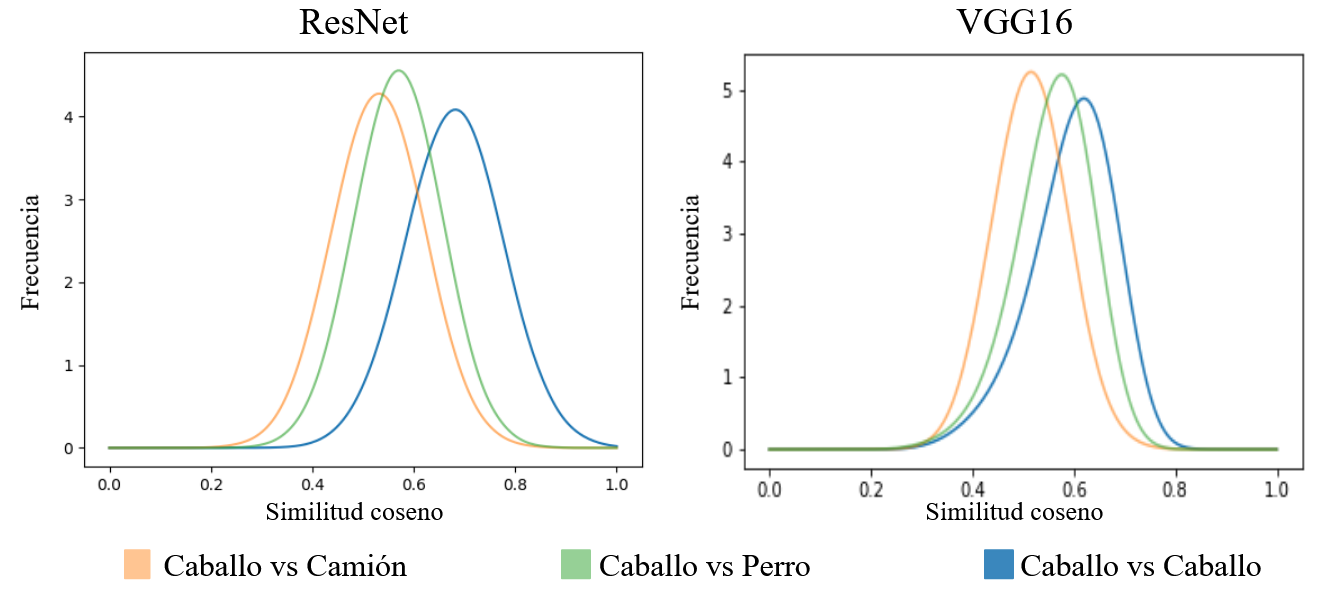
\includegraphics[width=1\linewidth]{img/vgg-vs-resnet}
	\caption{Frecuencia de la similitud coseno de los vectores de caracteristicas visuales, ente la misma y distintas clases, para las CNN  \textbf{Inception ResNet V2} y \textbf{VGG16}.}
	\label{fig:vgg-vs-resnet}
\end{figure}

\section{Definición de métricas}
Entre los diferentes conjuntos de datos anotados utilizados por los desafíos de detección de objetos y la comunidad científica, la métrica más común utilizada para medir la precisión de las detecciones es el  \textbf{Mean Average Precision (mAP)}, seguida por \textbf{Recall}. Un problema que tienen la métricas en detección de objetos, es la fata de una implementación estándar para calcularlas. Ademas, aquellas implementaciones publicas, están muy encapsuladas al código y resulta muy difícil adaptarlo, para medir rendimientos de modelos propios. Como ya se menciono, el código de Bansal \cite{bansal2018zero} no esta disponible, por este motivo fue necesario encontrar alguna implementación de estas métricas. Se encontraron varias y luego de hacer cambios para utilizarlos, los resultados variaban mucho de un código a otro.
Fue asi que se encontró el trabajo de Padilla Rafael \cite{padilla2020survey}, que explica lo planteado:\\

\begin{center}
	 \textit{``La falta de consenso en diferentes trabajos e implementaciones de AP es un problema al que se enfrentan las comunidades académicas y científicas. Las implementaciones métricas escritas en diferentes lenguajes y plataformas computacionales generalmente se distribuyen con los conjuntos de datos correspondientes que comparten una descripción determinada del cuadro delimitador. De hecho, estos proyectos ayudan a la comunidad con las herramientas de evaluación, pero exigen trabajo adicional para adaptarse a otros conjuntos de datos y formatos de cuadro delimitador.''}\\
\end{center}

Ademas Padilla, propone una definición y un código para estandarizar las métricas, de esta manera se pueden comprar distintos modelos, de una forma ``justa''. Por estos motivos decidimos utilizar este trabajo, aunque los resultados de nuestros modelos, no sean exactos a los reportados por Bansal \cite{bansal2018zero}.\\

Ahora definamos las métricas, basándonos en el trabajo \cite{padilla2020survey}. Primero es necesario, estandarizar cuando un cuadro es:
\begin{itemize}
	\item Falso negativo (\textbf{FN}): No se obtuvo ninguna detección en absoluto, o para un cuadro delimitador verdadero el IoU $> 0.5$ y no se predijo correctamente la clase
	\item Falso positivo (\textbf{FP}): Para un cuadro delimitador verdadero, se predijo correctamente la clase pero el IoU $< 0.5$, o es un predicción duplicada, es decir, ya se marco otra con mayor IOU como \textbf{TP}.
	\item Verdadero positivo (\textbf{TP}): Para un cuadro delimitador verdadero, se obtuvo  una propuesta con un IoU $> 0.5$ y se predijo correctamente la clase.
	\item Verdadero negativo (\textbf{TN}): Esto solo tiene sentido si, se quisiera medir propuestas que no tenían un IoU $> 0.5$ con todos los cuadros verdaderos, y ademas se predijo como clase de fondo. Pero en este trabajo no es utilizada.
\end{itemize}


La \textbf{Recall}, también conocida como sensibilidad, mide la probabilidad de que los objetos verdaderos (los que se encuentran en la imagen) se detecten correctamente, viene dado por: \[Recall =\frac{TP}{FN+TP}\] El trabajo de Bansal, define Recall de la siguiente manera: 
\begin{center}
	\textit{``Un cuadro delimitador predicho se marca como verdadero positivo solo si tiene una superposición de IoU mayor que un cierto umbral t con un cuadro delimitador de verdad del terreno y no se ha asignado ningún otro cuadro delimitador de mayor confianza al mismo cuadro de verdad del terreno. De lo contrario, se marca como falso positivo.''}\\
\end{center}

Según lo que se puede interpretar, utiliza los falsos positivos para calcular la \textbf{recall} en ves de usar Falso negativo. Sin poner en tela de juicio, si esto esta bien o mal, es claro que de esta forma solo se tiene en cuenta, los objetos que tuvieron al menos una propuesta con un IoU $> 0.5$ y el resto, quedan fuera del calculo de esta métrica. Esto genera una diferencia enorme en los resultados y dificulta la tarea de comprar con otros modelos, es  por esto que en este trabajo reportamos ambas. Bansal ademas, calcula una variación denominada K@Recall, donde solo se tienen en cuentan las K mejores propuestas basándose en la confianza de la predicción y el resto son descartadas.\\

\begin{equation} 
	\label{eqn:precision}
	Precision =\frac{TP}{FP+TP}
\end{equation}

AP, es una métrica popular para evaluar la precisión de los detectores de objetos mediante la estimación del área bajo la curva (AUC) de la relación \textbf{precisión} \ref{eqn:precision} x \textbf{recall}. La curva de \textbf{precisión} x \textbf{recall} puede verse como una compensación entre ambas métricas para diferentes valores de confianza asociados a los cuadros delimitadores generados por un detector. Si la confianza de un detector es tal que su FP es bajo, la precisión será alta. Sin embargo, en este caso, se pueden pasar por alto muchos aspectos positivos, lo que produce un FN alto y, por lo tanto, una recall baja. Por el contrario, si uno acepta más positivos, el recuerdo aumentará, pero el FP también puede aumentar, disminuyendo la precisión. Sin embargo, un buen detector de objetos debe encontrar todos los objetos reales  mientras identifica solo los objetos relevantes . Por lo tanto, un detector de objetos en particular puede considerarse bueno si su precisión permanece alta a medida que aumenta su recuperación, lo que significa que si el umbral de confianza varía, la precisión y la recall seguirán siendo altas. Por lo tanto, un área alta bajo la curva (AUC) tiende a indicar tanto una alta precisión como una alta recuperación. \textbf{mAP} para la detección de objetos es el promedio del AP calculado para todas las clases. Por lo general también se indica sobre que IoU se calcula, por ejemplo, mAP@0.5, o un conjunto de umbrales como mAP@[x, y]. El trabajo de Bansal reporta \textbf{mAP}, pero no indica sobre que IoU se calcula, a si que se asume que utilizo un valor de 0,5. Muchos trabajos que utilizan COCO, reportan mAP@[.5, .95]. Esta métrica resulta muy útil si se quiere comparar rendimientos entre distinto trabajos.


\section{Detalles de metodología de evaluación}
El principal experimento consto en replicar los resultados de Bansal \cite{bansal2018zero}. No se realizo exactamente sus experimentos, ya que esto no aportaría nada nuevo. Así que, se decidió analizar sus resultados y solo replicar los que consideramos indispensable y que seria un buen punto de partida. Por ejemplo, los experimentos con clases de fondo, no obtuvieron buenos resultados, en comparación con los que no la utiliza. Es por esto que no consideramos realizaros. El principal objetivo fue obtener un modelo que obtenga resultados lo mas similar posible a los reportados. Después de varias iteraciones, no se pudo lograr, y el principal motivo es la falta de una implementación para calcular las métricas. Se utiliza el código desarrollado por \cite{padilla2020survey}, pero sin ninguna garantía de que las métricas se calculen de la misma manera.\\

Ahora definamos la metodología de evaluación. El primer paso consiste generar propuestas para cada imagen, luego cada cuadro propuesto es reescalado al tamaño de la capa de entrada que tiene la CNN, y se le extrae el vector de características visuales. Después, se utiliza el modelo entrenado para inferir el vector de características semánticas, y se calcula la similitud coseno con los vectores semánticos de todas las clases o solo las invisibles, dependiendo si se quiere evaluar ZSDG o ZSD. Aquella clase que obtenga el mayor puntaje es asignada a la propuesta. También, se guarda la puntuación como la confianza de predicción.  Por ultimo, se agrupan todas las propuestas que se tengan asignada la misma clase y se corre un algoritmo de supresión no máxima. NMS elimina las predicciones repetidas y retorna las mejores propuestas de cada grupo. Al final obtenemos como resultado un conjunto de propuestas, sus clases y su respectivo puntaje. Estos datos se guardan en un archivo y luego se corre la implementación de Padilla, para obtener los resultados de las métricas.\\


